\documentclass[12pt]{article}

\usepackage[utf8]{inputenc}
\usepackage[russian]{babel}
\usepackage{amsmath}
\usepackage{setspace}

\usepackage{caption}
\usepackage{subcaption}
\usepackage{float}
\usepackage{graphicx}
\graphicspath{ {./images/} }

\usepackage{geometry}
 \geometry{
 a4paper,
 left=20mm,
 right=20mm,
 top=20mm,
 bot=20mm,
 }

\begin{document}

\begin{titlepage}
\begin{center}
    {\small НАЦИОНАЛЬНЫЙ ИССЛЕДОВАТЕЛЬСКИЙ УНИВЕРСИТЕТ ИТМО} \\
    {\small Факультет систем управления и робототехники} \\
    \vspace*{10\baselineskip}
    {\LARGEЭлектроника и схемотехника} \\
    \ \\
    \begin{spacing}{1.5}
    {\large Лабораторная работа №5 \\
    Исследование работы инвентирующего и неинвентирующего усилителя} \\
    \end{spacing} \\
    \ \\
    Вариант 2 \\
    \vspace*{10\baselineskip}
    \hfill {Выполнили студенты:} \\
    \hfill {Кирбаба Д.Д. R3338} \\
    \hfill {Курчавый В.В. R3338} \\
    \ \\
    \hfill {Преподаватель:} \\
    \hfill {Николаев Н.А.} \\
    \mbox{}
    \vfill {г. Санкт-Петербург\\2023}
\end{center}
\end{titlepage}

\section*{Цель работы}
\begin{itemsize}
    \item Изучение основных свойств и режимов работы операционных усилителей;
    \item Знакомство с типовыми схемами использования операционного усилителя;
    \item Анализ типовых схем включения в программном пакете LtSpice;
    \item Экспериментальное определение параметров усилителя в различных схемах включения.
\end{itemsize}

\section*{Ход работы}
Вариант 2.\\
Параметры усилителя:
\[
    R_{fb} = 50 \ kOhm, \ K = 10.
\]

\subsubsection*{Построение передаточной характеристики инвертирующего усилителя}
Рассчитаем величину сопротивления резистора: $R_1 = \frac{R_fb}{K} = 5 \ kOhm.$
\begin{figure}[H]
    \centering
    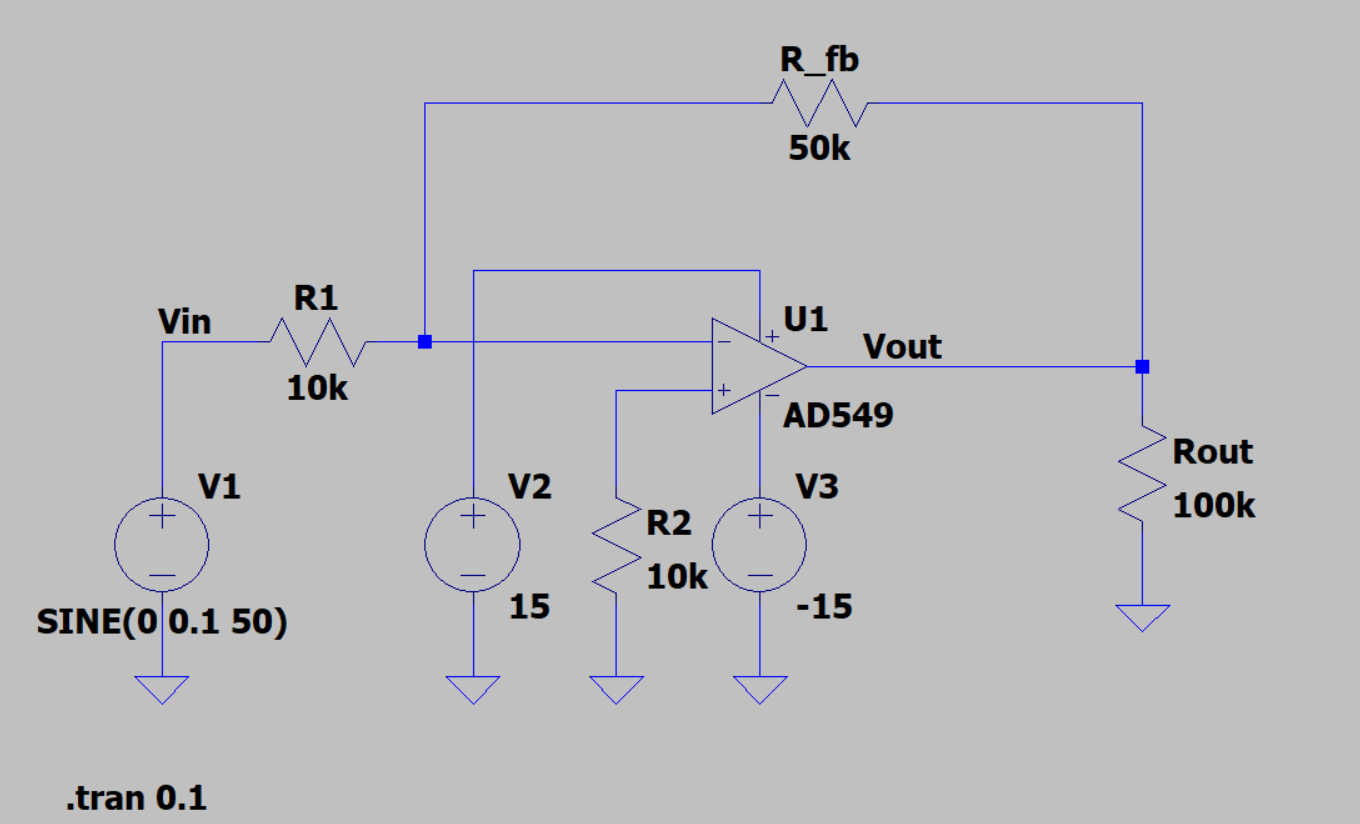
\includegraphics[width=0.7\textwidth]{1_scheme.png}
    \caption{Принципиальная схема инвертирующего усилителя на ОУ.}
    \label{fig:1_scheme}
\end{figure}

Снимем передаточную характеристику инвертирующего усилителя:
\begin{figure}[H]
    \centering
    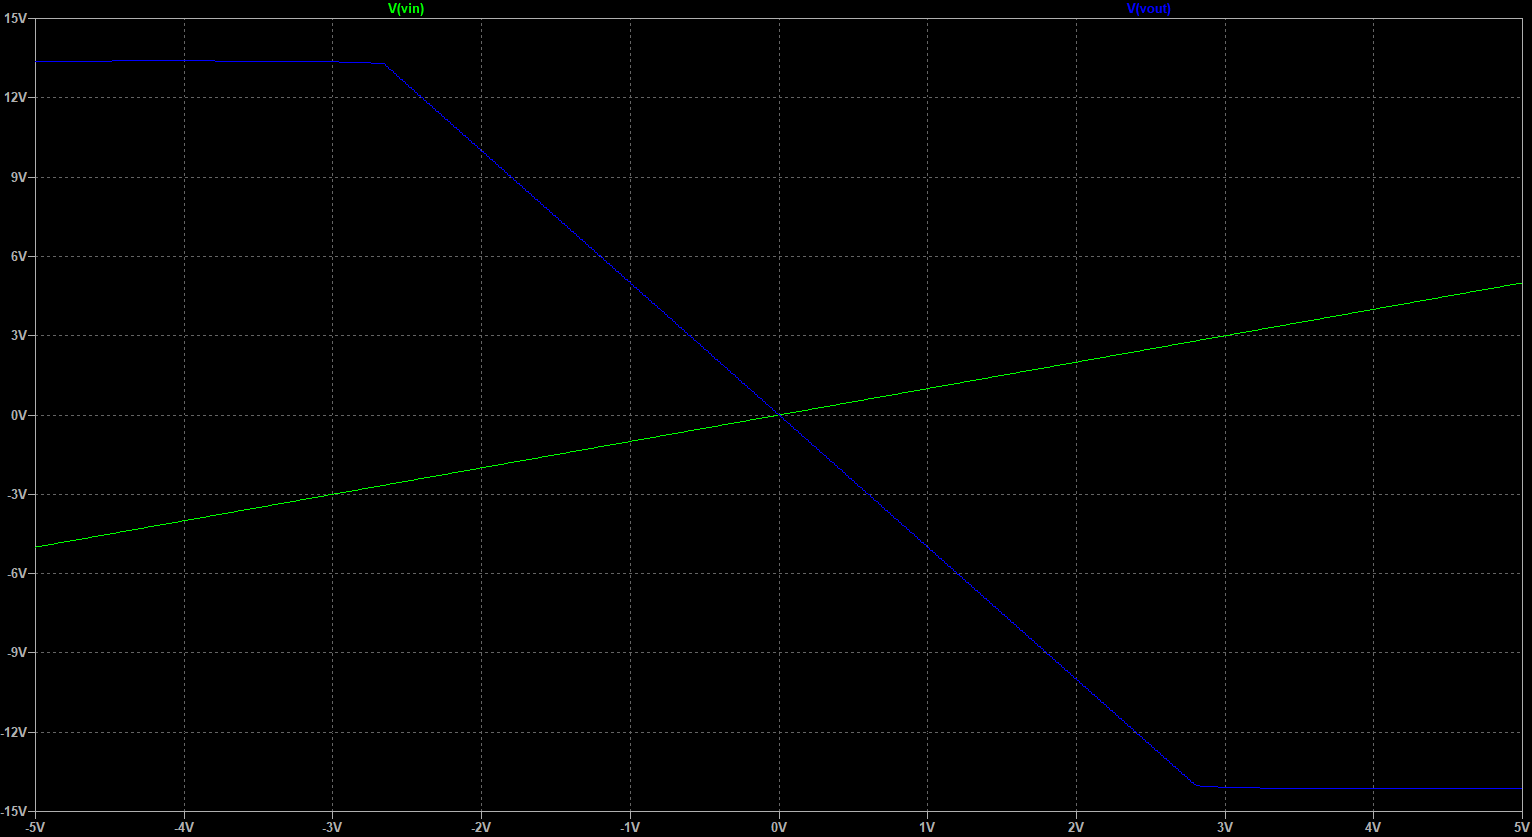
\includegraphics[width=\textwidth]{1_in_out.png}
    \caption{Передаточная характеристика инвертирующего усилителя.}
    \label{fig:1_in_out}
\end{figure}

Определим по графикам положительное и отрицательное напряжения ограничения:
\[
    V_{lim+} = 13.391 \ V, \ V_{lim-} = -14.1347 \ V.
\]
Рассчитаем коэффициент усиления:
\[
    (V_{in_1} = -2 \ V, \ V_{out_1} = 9.9999 \ V), \ (V_{in_2} = 2 \ V, \ V{out_2} = -9.9999).
\]
\[
    K = \frac{V_{out_2} - V_{out_1}}{V_{in_2} - V_{in_1}} = -4.99995.
\]

\subsubsection*{Исследование работы инвентирующего усилителя}
\begin{figure}[H]
    \centering
    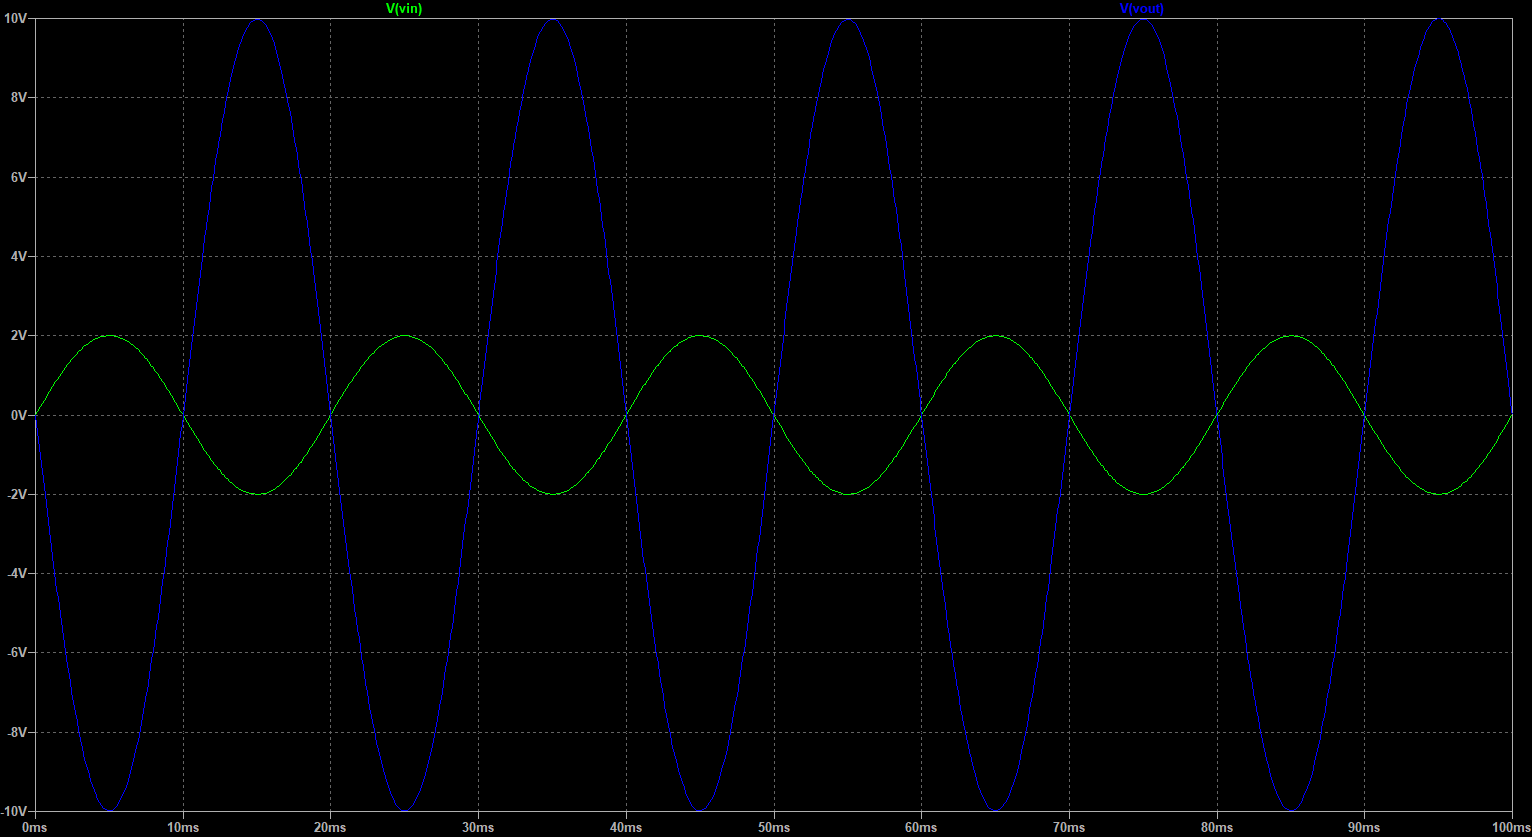
\includegraphics[width=\textwidth]{1_sin_in_out.png}
    \caption{Инвентирующий усилитель при синусоидальном сигнале.}
    \label{fig:1_sin_in_out}
\end{figure}
Фазы входного и выходного сигналов находятся в противофазе ($pi$). \\
Инвентирующий усилитель изменяет полярность сигнала. \\
Определим коэффициент усиления:
\[
    K = \frac{V_{out_{amp_{max}}}}{V_{in_{amp_{max}}}} = -5.
\]
Значение вычисленного коэффициента совпало с вычисленным значением из предыдущего пункта.

\subsubsection*{Построение передаточной характеристики неинвертирующего усилителя}
Рассчитаем величину сопротивления резистора: $R_1 = \frac{R_fb}{K-1} = 5.555 \ kOhm.$
\begin{figure}[H]
    \centering
    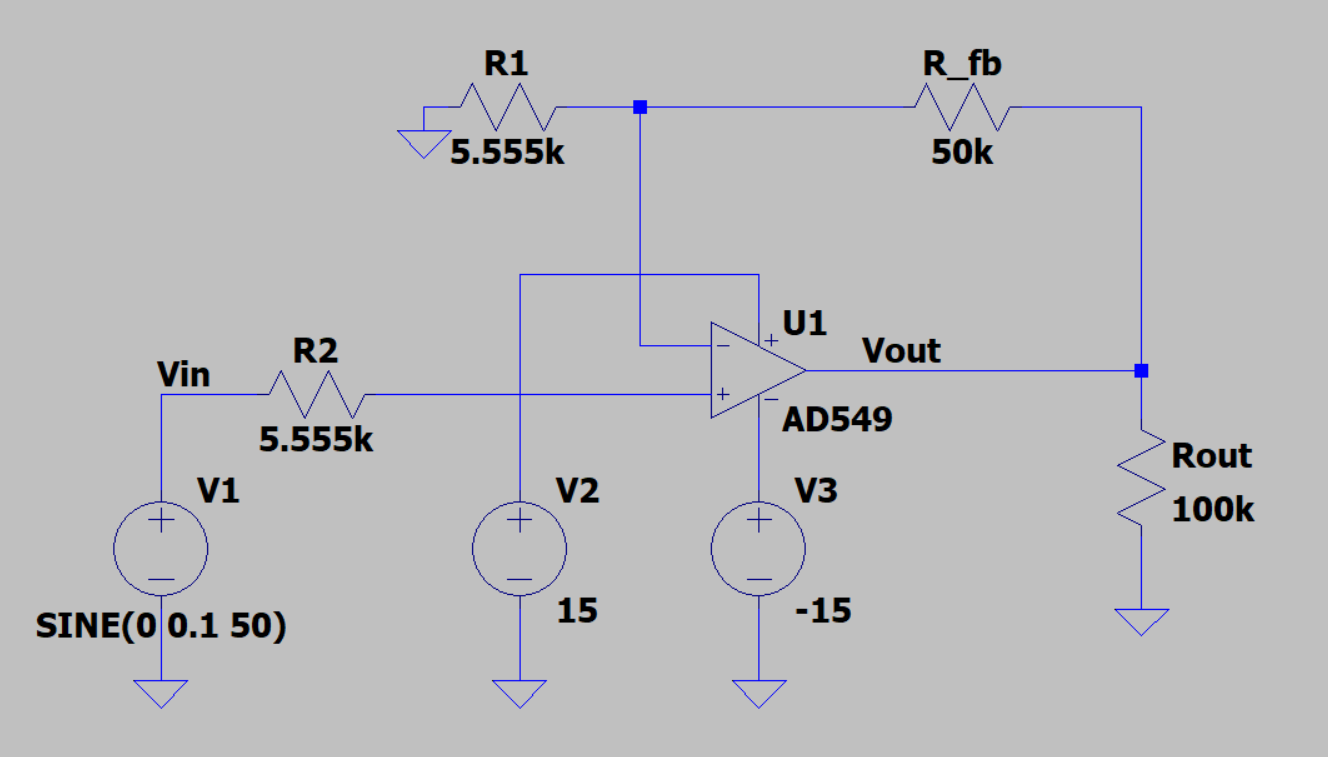
\includegraphics[width=0.7\textwidth]{2_scheme.png}
    \caption{Принципиальная схема неинвертирующего усилителя на ОУ.}
    \label{fig:2_scheme}
\end{figure}

Снимем передаточную характеристику неинвертирующего усилителя:
\begin{figure}[H]
    \centering
    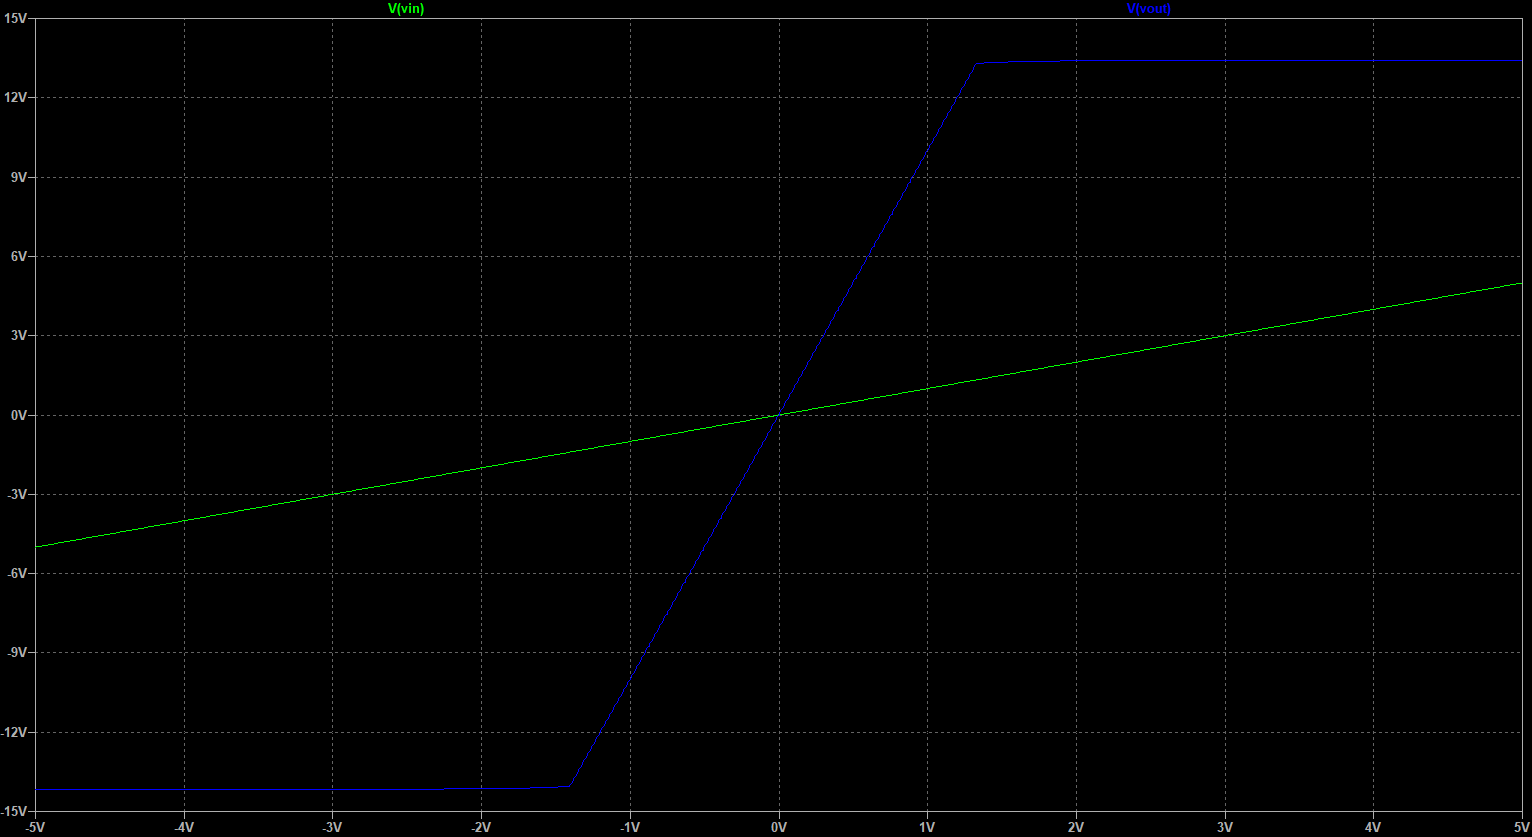
\includegraphics[width=\textwidth]{2_in_out.png}
    \caption{Передаточная характеристика неинвертирующего усилителя.}
    \label{fig:2_in_out}
\end{figure}

Определим по графикам положительное и отрицательное напряжения ограничения:
\[
    V_{lim+} = 13.407 \ V, \ V_{lim-} = -14.154 \ V.
\]
Рассчитаем коэффициент усиления:
\[
    (V_{in_1} = -1 \ V, \ V_{out_1} = -10.0008 \ V), \ (V_{in_2} = 1 \ V, \ V{out_2} = 10.0008).
\]
\[
    K = \frac{V_{out_2} - V_{out_1}}{V_{in_2} - V_{in_1}} = 10.0008.
\]

\subsubsection*{Исследование работы неинвентирующего усилителя}
\begin{figure}[H]
    \centering
    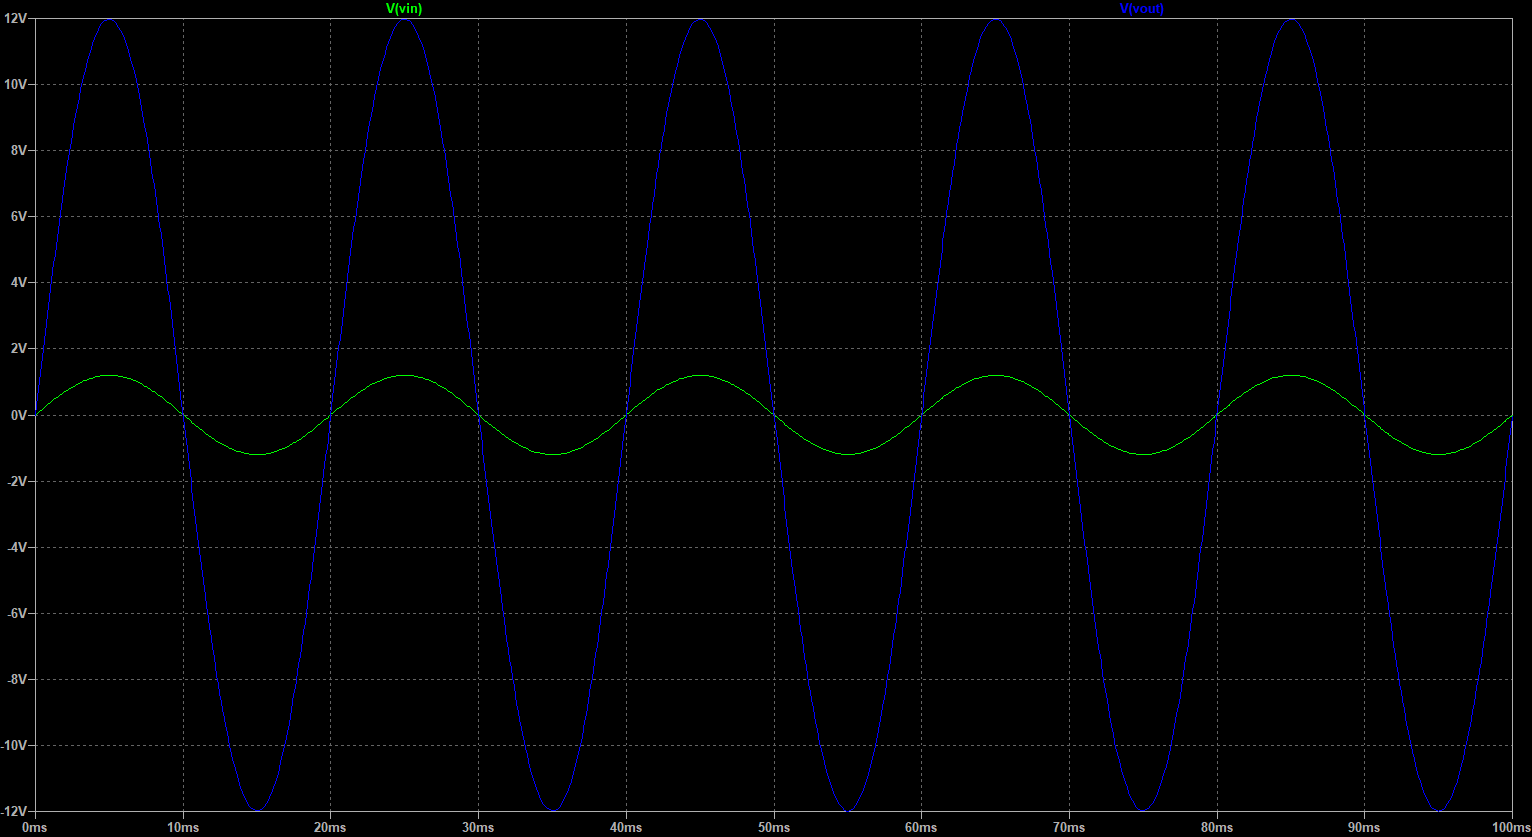
\includegraphics[width=\textwidth]{2_sin_in_out.png}
    \caption{Неинвентирующий усилитель при синусоидальном сигнале.}
    \label{fig:2_sin_in_out}
\end{figure}
Фазы входного и выходного сигналов совпадают по фазе. \\
Инвентирующий усилитель не изменяет полярность сигнала. \\
Определим коэффициент усиления:
\[
    K = \frac{V_{out_{amp_{max}}}}{V_{in_{amp_{max}}}} = 10.
\]
Значение вычисленного коэффициента совпало с вычисленным значением из предыдущего пункта.
\section*{Выводы}
В данной лабораторной работе были исследованы операционные усилители. Их цель - усиление напряжения и обеспечивание выполнения различных операций по преобразованию аналоговых электрических сигналов. \\
ОУ обычно обладает следующими свойствами: дифференциальным входом, большим коэффициентом усиления $K$, малыми входными токами $I_{in}$, большим входным сопротивлением $R_{in}$, малым выходным сопротивлением $R_{out}$. \\
Так как ОУ содержит в себе дифференциальный усилитель, то он реагирует только на разность входных токов, а следовательно является достаточной устойчивым прибором (т.к. изменение температуры и старение деталей транзисторов можно рассматривать как синфазные входные воздействия). \\
В схему ОУ обязательно добавляют обратную связь для стабилизации коэффициента усиления, уменьшения искажений и расширения диапазона усиливаемых частот.
\ \\
При исследовании усилителей были построены их схемы, промоделирована работа как на постоянном, так и на синусоидальном входном воздействии. Коэффициенты усилений оказались равны в обоих случаях: $K_{inv} = -5, \ K{dir} = 10$. \\
Также по графикам переходных процессов были определены напряжения ограничений, они, как и предполагалось, оказались меньше на $1-2 \ V$ от напряжения питания усилителей.

\end{document}